% =====================================================================
%  Capítulo 6. Modelos ARMA
% =====================================================================
\chapter[Modelos ARMA]{Modelos ARMA: identificación, estimación, diagnóstico y pronóstico}\label{cap:arma}

\section*{Objetivos de aprendizaje}
Al terminar este capítulo, el lector podrá:
\begin{enumerate}[label=\arabic*.,leftmargin=*]
  \item Derivar los momentos y la función de autocorrelación de los procesos MA, AR y ARMA, y reconocer sus
        patrones en la ACF y la PACF.
  \item Estimar modelos ARMA por máxima verosimilitud, elegir entre ellos con criterios de información y
        diagnosticar sus residuos.
  \item Cuantificar el sesgo de muestras finitas del estimador autorregresivo y su consecuencia en las
        regresiones predictivas (sesgo de Stambaugh).
  \item Construir pronósticos puntuales y por intervalos, y evaluarlos fuera de muestra con la prueba de
        Diebold-Mariano.
\end{enumerate}

\section*{Motivación}
El Capítulo~\ref{cap:raiz} enseñó a decidir si una serie es estacionaria. Si lo es, la siguiente pregunta es
cómo depende de su pasado. Los modelos ARMA (autorregresivos y de medias móviles) de Box y Jenkins (1970) son
la respuesta clásica: describen la dependencia de una serie estacionaria con pocos parámetros, y con ellos se
pronostica. En finanzas no sirven para predecir la dirección de los precios (los rendimientos son casi ruido
blanco), pero sí para variables persistentes como la volatilidad implícita, las tasas de interés, los
diferenciales de crédito o la inflación, y para entender los artefactos de los datos, como el efecto de
Working.

\paragraph{Datos del capítulo.} Cambios mensuales del rendimiento del bono del Tesoro de EE.\,UU. a 10 años
(1953--2023), logaritmo del VIX diario (1990--2026) y la razón dividendo/precio del S\&P 500 (1946--2023). La
tasa de interés se usa desde 1953, cuando ya regía el acuerdo de 1951 entre el Tesoro y la Reserva Federal
que dejó las tasas largas en manos del mercado.

% ---------------------------------------------------------------------
\section{Procesos de medias móviles}
% ---------------------------------------------------------------------

Usaremos el \emph{operador de rezagos} $L$, definido por $Ly_t=y_{t-1}$ y $L^jy_t=y_{t-j}$.

\begin{definicion}[MA($q$)]
Un proceso de medias móviles de orden $q$ es
\[
  y_t=\mu+\varepsilon_t+\theta_1\varepsilon_{t-1}+\cdots+\theta_q\varepsilon_{t-q}=\mu+\theta(L)\,\varepsilon_t,
\]
con $\varepsilon_t$ ruido blanco de varianza $\sigma^2$ y $\theta(L)=1+\theta_1L+\cdots+\theta_qL^q$.
\end{definicion}

\begin{proposicion}[Momentos del MA(1)]\label{prop:ma1}
Para $y_t=\mu+\varepsilon_t+\theta\varepsilon_{t-1}$:
\begin{align*}
  \E[y_t]  &= \mu,\\
  \gamma_0 &= \sigma^2(1+\theta^2),\\
  \gamma_1 &= \theta\,\sigma^2,\\
  \gamma_j &= 0 \quad (j\ge2),\\
  \rho_1   &= \frac{\theta}{1+\theta^2}.
\end{align*}
\end{proposicion}

\begin{proof}
La media es inmediata. Para las autocovarianzas, como los $\varepsilon$ no están correlacionados, solo
contribuyen los términos con el mismo subíndice:
\begin{align*}
  \gamma_0 &= \Var(\varepsilon_t+\theta\varepsilon_{t-1})\\
           &= \sigma^2+\theta^2\sigma^2\\
           &= \sigma^2(1+\theta^2),\\
  \gamma_1 &= \Cov(\varepsilon_t+\theta\varepsilon_{t-1},\ \varepsilon_{t-1}+\theta\varepsilon_{t-2})\\
           &= \theta\,\Var(\varepsilon_{t-1})\\
           &= \theta\,\sigma^2 .
\end{align*}
Para $j\ge2$, $y_t$ y $y_{t-j}$ no comparten ningún choque y $\gamma_j=0$. Por último,
$\rho_1=\gamma_1/\gamma_0=\theta/(1+\theta^2)$.
\end{proof}

La ACF de un MA($q$) se \emph{corta} después del rezago $q$: es la firma que permite identificarlo. La
Proposición tiene dos consecuencias.

\begin{corolario}\label{cor:ma1cota}
(a) En un MA(1), $|\rho_1|\le\tfrac12$. (b) Los valores $\theta$ y $1/\theta$ producen la misma $\rho_1$.
\end{corolario}

\begin{proof}
(a) Como $(1-|\theta|)^2\ge0$:
\begin{align*}
  1-2|\theta|+\theta^2 &\ge 0\\
  1+\theta^2           &\ge 2|\theta|\\
  \frac{|\theta|}{1+\theta^2} &\le \frac12 .
\end{align*}
(b) Sustituyendo $1/\theta$ en la fórmula y multiplicando numerador y denominador por $\theta^2$:
\begin{align*}
  \frac{1/\theta}{1+1/\theta^2} &= \frac{\theta}{\theta^2+1}. && \qedhere
\end{align*}
\end{proof}

Por (b), un mismo patrón de autocorrelación es compatible con dos valores de $\theta$. Se elige el que cumple
$|\theta|<1$, llamado \emph{invertible}, porque solo con él se pueden recuperar los choques pasados a partir de
los datos: $\varepsilon_t=\sum_{j\ge0}(-\theta)^j(y_{t-j}-\mu)$, una suma que converge solo si $|\theta|<1$.

\begin{proposicion}[El MA(1) del efecto de Working]\label{prop:workingma}
Los cambios de una serie promediada a partir de un paseo aleatorio tienen $\rho_1=1/4$ y $\rho_j=0$ para
$j\ge2$ (Proposición~\ref{prop:working}). Su representación MA(1) invertible tiene
\[
  \theta=2-\sqrt3\approx0{,}268 .
\]
\end{proposicion}

\begin{proof}
Igualamos $\rho_1$ del MA(1) a $1/4$ y resolvemos la ecuación de segundo grado en $\theta$:
\begin{align*}
  \frac{\theta}{1+\theta^2} &= \frac14\\
  4\theta                   &= 1+\theta^2\\
  \theta^2-4\theta+1        &= 0\\
  \theta                    &= \frac{4\pm\sqrt{16-4}}{2}\\
                            &= 2\pm\sqrt3 .
\end{align*}
Las raíces son $2+\sqrt3\approx3{,}73$ y $2-\sqrt3\approx0{,}268$, una inversa de la otra; la invertible es la
segunda.
\end{proof}

% ---------------------------------------------------------------------
\section{Procesos autorregresivos y ARMA}
% ---------------------------------------------------------------------

\begin{definicion}[AR($p$) y ARMA($p,q$)]
Un AR($p$) es $\phi(L)\,y_t=c+\varepsilon_t$ con $\phi(L)=1-\phi_1L-\cdots-\phi_pL^p$. Un ARMA($p,q$) es
$\phi(L)\,y_t=c+\theta(L)\,\varepsilon_t$. El proceso es estacionario si todas las raíces de $\phi(z)=0$ están
fuera del círculo unitario ($|z|>1$), e invertible si lo están las de $\theta(z)=0$.
\end{definicion}

Para el AR(1), la condición se reduce a $|\phi|<1$: la raíz de $1-\phi z=0$ es $z=1/\phi$.

\begin{proposicion}[Ecuaciones de Yule-Walker del AR(2)]\label{prop:ar2}
En un AR(2) estacionario, $y_t=c+\phi_1y_{t-1}+\phi_2y_{t-2}+\varepsilon_t$,
\begin{align*}
  \rho_1 &= \frac{\phi_1}{1-\phi_2},\\
  \rho_j &= \phi_1\,\rho_{j-1}+\phi_2\,\rho_{j-2} \quad (j\ge2).
\end{align*}
\end{proposicion}

\begin{proof}
Trabajamos con la serie centrada, $\tilde y_t=y_t-\mu$, que cumple
$\tilde y_t=\phi_1\tilde y_{t-1}+\phi_2\tilde y_{t-2}+\varepsilon_t$. Multiplicamos por $\tilde y_{t-j}$ con
$j\ge1$ y tomamos esperanzas; como $\varepsilon_t$ no está correlacionado con el pasado,
\begin{align*}
  \E[\tilde y_t\,\tilde y_{t-j}] &= \phi_1\,\E[\tilde y_{t-1}\,\tilde y_{t-j}]+\phi_2\,\E[\tilde y_{t-2}\,\tilde y_{t-j}]\\
  \gamma_j                       &= \phi_1\,\gamma_{j-1}+\phi_2\,\gamma_{j-2}\\
  \rho_j                         &= \phi_1\,\rho_{j-1}+\phi_2\,\rho_{j-2}.
\end{align*}
Con $j=1$, usando $\rho_0=1$ y $\rho_{-1}=\rho_1$:
\begin{align*}
  \rho_1               &= \phi_1+\phi_2\,\rho_1\\
  \rho_1\,(1-\phi_2)   &= \phi_1\\
  \rho_1               &= \frac{\phi_1}{1-\phi_2}. && \qedhere
\end{align*}
\end{proof}

Si las raíces de $\phi(z)$ son complejas, como con $\phi_1=1{,}2$ y $\phi_2=-0{,}5$, la recursión de
Yule-Walker produce una ACF que oscila mientras decae, el patrón típico de los ciclos.

\begin{proposicion}[ACF del ARMA(1,1)]\label{prop:arma11}
Para $y_t=\phi\,y_{t-1}+\varepsilon_t+\theta\varepsilon_{t-1}$ (centrado) con $|\phi|<1$:
\begin{align*}
  \gamma_0 &= \sigma^2\,\frac{1+2\phi\theta+\theta^2}{1-\phi^2},\\
  \rho_1   &= \frac{(1+\phi\theta)(\phi+\theta)}{1+2\phi\theta+\theta^2},\\
  \rho_j   &= \phi\,\rho_{j-1} \quad (j\ge2).
\end{align*}
\end{proposicion}

\begin{proof}
Necesitamos dos covarianzas auxiliares. Como $y_{t-1}$ no depende de $\varepsilon_t$:
\begin{align*}
  \E[y_t\,\varepsilon_t]     &= \E[\varepsilon_t^2] = \sigma^2,\\
  \E[y_t\,\varepsilon_{t-1}] &= \phi\,\E[y_{t-1}\varepsilon_{t-1}]+\theta\,\E[\varepsilon_{t-1}^2]\\
                             &= (\phi+\theta)\,\sigma^2 .
\end{align*}
Multiplicando la ecuación del modelo por $y_t$ y por $y_{t-1}$ y tomando esperanzas:
\begin{align*}
  \gamma_0 &= \phi\,\gamma_1+\sigma^2+\theta(\phi+\theta)\,\sigma^2, \tag{a}\\
  \gamma_1 &= \phi\,\gamma_0+\theta\,\sigma^2 . \tag{b}
\end{align*}
Sustituyendo (b) en (a):
\begin{align*}
  \gamma_0           &= \phi^2\gamma_0+\phi\theta\sigma^2+\sigma^2+\phi\theta\sigma^2+\theta^2\sigma^2\\
  \gamma_0(1-\phi^2) &= \sigma^2\,(1+2\phi\theta+\theta^2)\\
  \gamma_0           &= \sigma^2\,\frac{1+2\phi\theta+\theta^2}{1-\phi^2}.
\end{align*}
Volviendo a (b):
\begin{align*}
  \gamma_1 &= \sigma^2\,\frac{\phi(1+2\phi\theta+\theta^2)+\theta(1-\phi^2)}{1-\phi^2}\\
           &= \sigma^2\,\frac{\phi+\theta+\phi^2\theta+\phi\theta^2}{1-\phi^2}\\
           &= \sigma^2\,\frac{(1+\phi\theta)(\phi+\theta)}{1-\phi^2}.
\end{align*}
Dividiendo $\gamma_1$ entre $\gamma_0$ se obtiene $\rho_1$. Para $j\ge2$, el término de media móvil ya no
está correlacionado con $y_{t-j}$ y queda $\gamma_j=\phi\,\gamma_{j-1}$.
\end{proof}

\subsection{Identificación}

La Tabla~\ref{tab:identificacion} y la Figura~\ref{fig:identificacion} resumen los patrones teóricos que guían
la elección inicial del modelo. En la práctica las ACF y PACF muestrales son ruidosas y varios modelos pueden
ser compatibles con ellas; la elección final se hace con criterios de información y diagnóstico de residuos.

\begin{table}[ht]
\centering\small
\begin{tabular}{@{}lll@{}}
\toprule
Modelo & ACF & PACF \\
\midrule
AR($p$)       & decae (geométrica u oscilante) & se corta después de $p$ \\
MA($q$)       & se corta después de $q$        & decae \\
ARMA($p,q$)   & decae a partir de $q$          & decae a partir de $p$ \\
\bottomrule
\end{tabular}
\caption{Patrones de identificación de Box y Jenkins.}
\label{tab:identificacion}
\end{table}

\begin{figure}[ht]
\centering
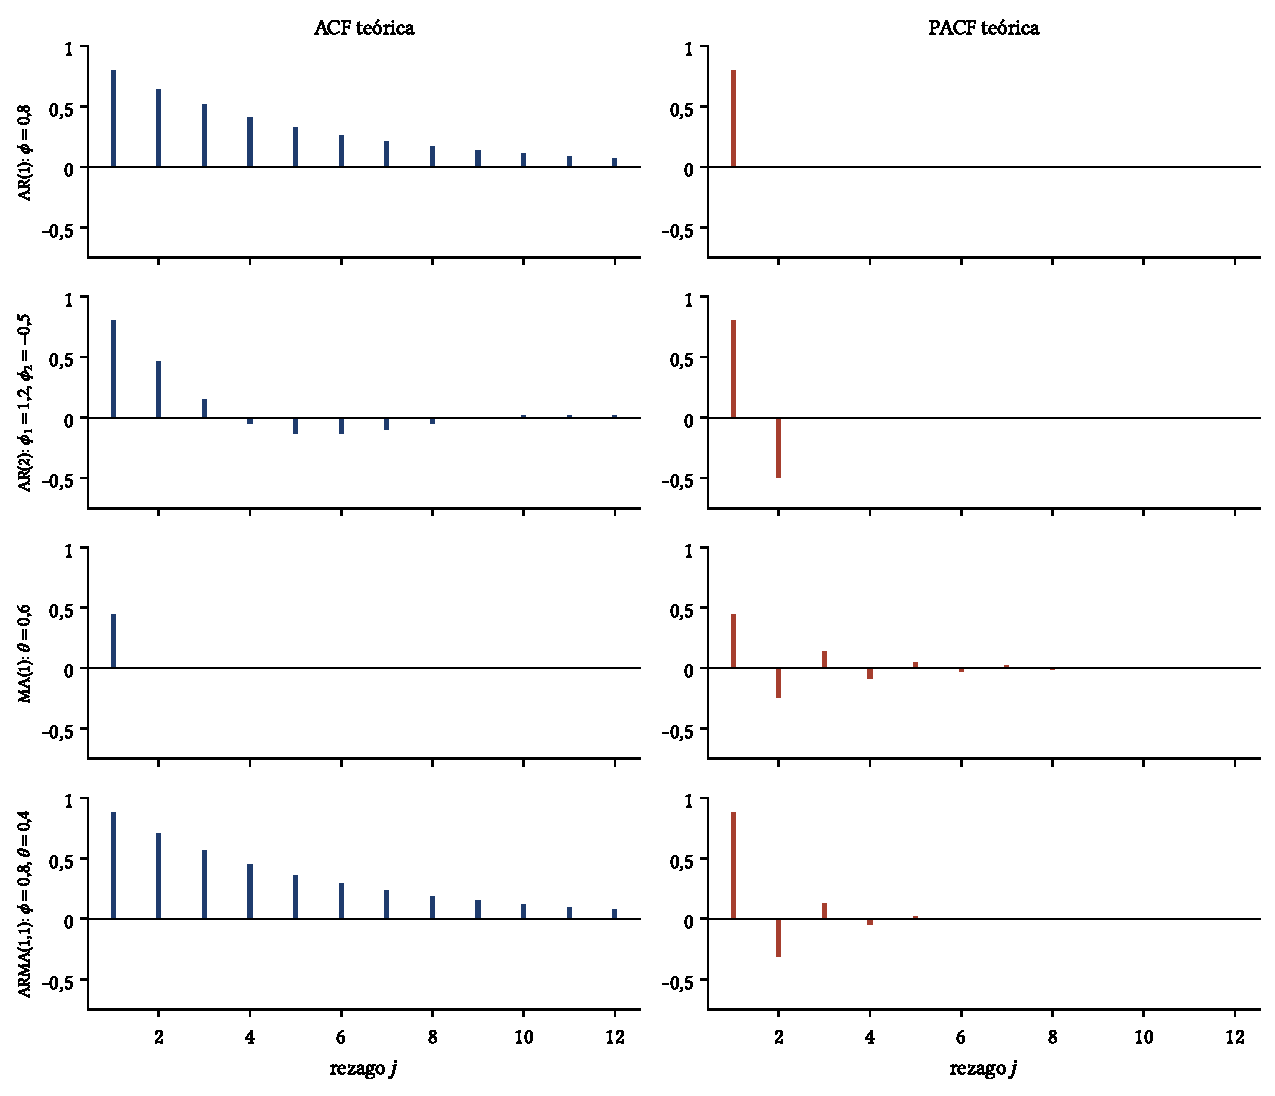
\includegraphics[width=0.92\linewidth]{graficos/cap06_fig_identificacion.pdf}
\caption{ACF (azul) y PACF (rojo) teóricas. El AR(1) tiene una ACF que decae geométricamente y una PACF con
una sola barra. El AR(2) con raíces complejas oscila. El MA(1) tiene una sola barra en la ACF y una PACF que
decae alternando de signo. El ARMA(1,1) combina ambos: las dos funciones decaen.}
\label{fig:identificacion}
\end{figure}

% ---------------------------------------------------------------------
\section{Estimación, selección y diagnóstico}
% ---------------------------------------------------------------------

\begin{proposicion}[MCO y máxima verosimilitud condicional en un AR]\label{prop:mvar}
Si $\varepsilon_t\sim N(0,\sigma^2)$, maximizar la verosimilitud del AR($p$) condicional en las primeras $p$
observaciones equivale a estimar por MCO la regresión de $y_t$ sobre una constante y $y_{t-1},\dots,y_{t-p}$.
\end{proposicion}

\begin{proof}
Condicional en el pasado, $y_t\sim N(c+\sum_j\phi_jy_{t-j},\ \sigma^2)$. La log-verosimilitud de
$y_{p+1},\dots,y_T$ es la suma de las log-densidades:
\begin{align*}
  \ell(c,\bm\phi,\sigma^2) &= \sum_{t=p+1}^T\Bigl[-\tfrac12\ln(2\pi\sigma^2)
                              -\frac{\bigl(y_t-c-\sum_j\phi_jy_{t-j}\bigr)^2}{2\sigma^2}\Bigr]\\
                           &= -\frac{T-p}{2}\ln(2\pi\sigma^2)-\frac{1}{2\sigma^2}\,\mathrm{SRC}(c,\bm\phi).
\end{align*}
Para cualquier $\sigma^2$, $\ell$ se maximiza en $(c,\bm\phi)$ minimizando $\mathrm{SRC}$, que es el problema
de MCO.
\end{proof}

Con términos de media móvil, los residuos dependen de los parámetros de forma no lineal
($\varepsilon_t=y_t-c-\phi y_{t-1}-\theta\varepsilon_{t-1}$), y la verosimilitud se maximiza numéricamente. R
(\texttt{arima}) y \texttt{statsmodels} (\texttt{ARIMA}) calculan la verosimilitud \emph{exacta} con el filtro
de Kalman; usan optimizadores distintos, por lo que sus estimaciones pueden diferir en la cuarta cifra
decimal.

\subsection{El sesgo de muestras finitas}

MCO es consistente en un AR(1) estacionario, pero sesgado en muestras finitas. Kendall (1954) mostró que, con
constante,
\[
  \E[\hat\phi]-\phi\approx-\frac{1+3\phi}{T}.
\]
El sesgo es negativo y crece con $\phi$: las series persistentes parecen menos persistentes de lo que son. La
Figura~\ref{fig:kendall} compara la fórmula con una simulación: es precisa hasta $\phi\approx0{,}9$ y
subestima el sesgo cerca de la raíz unitaria (con $\phi=0{,}99$ y $T=100$, la simulación da $-0{,}050$ y la
fórmula $-0{,}040$).

\begin{figure}[ht]
\centering
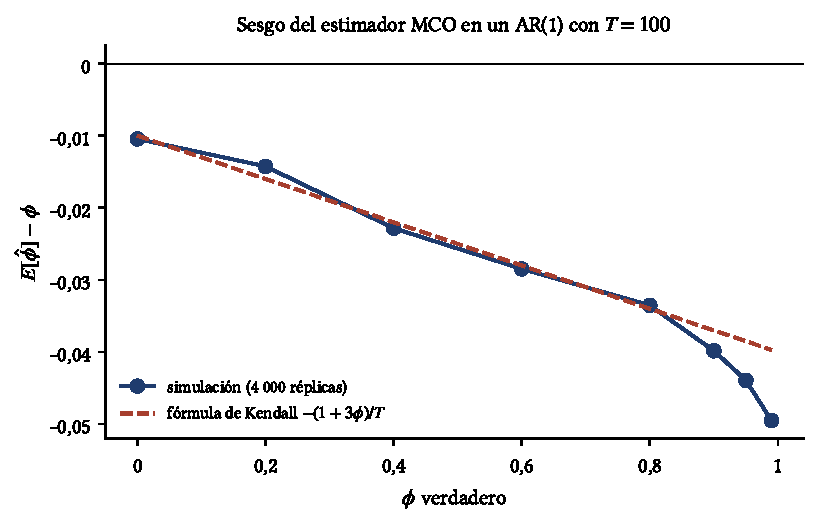
\includegraphics[width=0.72\linewidth]{graficos/cap06_fig_kendall.pdf}
\caption{Sesgo del estimador MCO de $\phi$ en un AR(1) con constante y $T=100$: simulación (puntos) y
aproximación de Kendall (línea discontinua).}
\label{fig:kendall}
\end{figure}

\begin{proposicion}[Sesgo de Stambaugh]\label{prop:stambaugh}
Considere la regresión predictiva y la dinámica del predictor
\begin{align*}
  r_{t+1} &= a+b\,x_t+u_{t+1},\\
  x_{t+1} &= c+\phi\,x_t+v_{t+1},
\end{align*}
con $(u_t,v_t)$ i.i.d. normales, de covarianza $\sigma_{uv}$, y $\sigma_v^2=\Var(v_t)$. Entonces
\[
  \E[\hat b-b]=\frac{\sigma_{uv}}{\sigma_v^2}\;\E[\hat\phi-\phi].
\]
\end{proposicion}

\begin{proof}
Proyectamos $u$ sobre $v$: $u_t=k\,v_t+\eta_t$ con $k=\sigma_{uv}/\sigma_v^2$ y $\eta_t$ independiente de toda
la sucesión $\{v_t\}$, y por tanto de toda la trayectoria de $x$. Con $S_{xx}=\sum_t(x_t-\bar x)^2$ y las sumas
sobre $t=1,\dots,T-1$, los estimadores MCO cumplen
\begin{align*}
  \hat b-b       &= \frac{\sum_t(x_t-\bar x)\,u_{t+1}}{S_{xx}},\\
  \hat\phi-\phi  &= \frac{\sum_t(x_t-\bar x)\,v_{t+1}}{S_{xx}}.
\end{align*}
Sustituyendo $u_{t+1}=k\,v_{t+1}+\eta_{t+1}$:
\begin{align*}
  \hat b-b &= k\,\frac{\sum_t(x_t-\bar x)\,v_{t+1}}{S_{xx}}+\frac{\sum_t(x_t-\bar x)\,\eta_{t+1}}{S_{xx}}\\
           &= k\,(\hat\phi-\phi)+\frac{\sum_t(x_t-\bar x)\,\eta_{t+1}}{S_{xx}} .
\end{align*}
Como $\eta$ es independiente de $x$, el segundo término tiene esperanza cero condicional en $x$. Tomando
esperanzas:
\begin{align*}
  \E[\hat b-b] &= k\,\E[\hat\phi-\phi]\\
               &= \frac{\sigma_{uv}}{\sigma_v^2}\,\E[\hat\phi-\phi]. && \qedhere
\end{align*}
\end{proof}

Con la razón dividendo/precio, $\sigma_{uv}<0$: cuando suben los precios, sube el rendimiento ($u>0$) y cae la
razón ($v<0$). Como $\E[\hat\phi-\phi]<0$, el sesgo de $\hat b$ es \emph{positivo}: la regresión exagera la
capacidad predictiva.

\subsection{Selección y diagnóstico}

Con $\hat\ell$ la log-verosimilitud maximizada y $k$ el número de parámetros, los criterios de información son
\[
  \mathrm{AIC}=-2\hat\ell+2k,\qquad \mathrm{BIC}=-2\hat\ell+k\ln T,
\]
y se elige el modelo con el menor valor. El BIC penaliza más los parámetros y, si el modelo verdadero está entre
los candidatos, lo elige con probabilidad que tiende a 1; el AIC tiende a elegir modelos algo más grandes, lo
que puede ser conveniente para pronosticar. Una vez elegido el modelo, sus residuos deben parecer ruido blanco:
se aplica la prueba de Ljung-Box con $m-p-q$ grados de libertad.

% ---------------------------------------------------------------------
\section{Pronóstico}
% ---------------------------------------------------------------------

El pronóstico que minimiza el error cuadrático medio es la esperanza condicional,
$\hat y_{T+h}=\E[y_{T+h}\mid y_T,y_{T-1},\dots]$.

\begin{proposicion}[Pronóstico de un AR(1)]\label{prop:pronar1}
En un AR(1) estacionario con media $\mu$:
\begin{align*}
  \hat y_{T+h} &= \mu+\phi^h\,(y_T-\mu),\\
  \E\bigl[(y_{T+h}-\hat y_{T+h})^2\bigr] &= \sigma^2\,\frac{1-\phi^{2h}}{1-\phi^2}.
\end{align*}
\end{proposicion}

\begin{proof}
Como en la Proposición~\ref{prop:vidamedia}, escribiendo $c=\mu(1-\phi)$:
\begin{align*}
  y_{T+h}-\mu &= \phi^h\,(y_T-\mu)+\sum_{i=0}^{h-1}\phi^{\,i}\,\varepsilon_{T+h-i}.
\end{align*}
Los choques futuros tienen esperanza condicional cero, de donde sale el pronóstico. El error es la suma de
choques futuros, que no están correlacionados:
\begin{align*}
  \E\bigl[(y_{T+h}-\hat y_{T+h})^2\bigr] &= \Var\Bigl(\sum_{i=0}^{h-1}\phi^{\,i}\,\varepsilon_{T+h-i}\Bigr)\\
                                         &= \sigma^2\sum_{i=0}^{h-1}\phi^{2i}\\
                                         &= \sigma^2\,\frac{1-\phi^{2h}}{1-\phi^2}. && \qedhere
\end{align*}
\end{proof}

Cuando $h\to\infty$, el pronóstico tiende a la media $\mu$ y el error cuadrático medio, a la varianza no
condicional $\sigma^2/(1-\phi^2)$: a horizontes largos, el mejor pronóstico es la media y el modelo ya no
aporta información. La Figura~\ref{fig:pronar1} muestra que la velocidad de ese proceso depende de $\phi$.

\begin{figure}[ht]
\centering
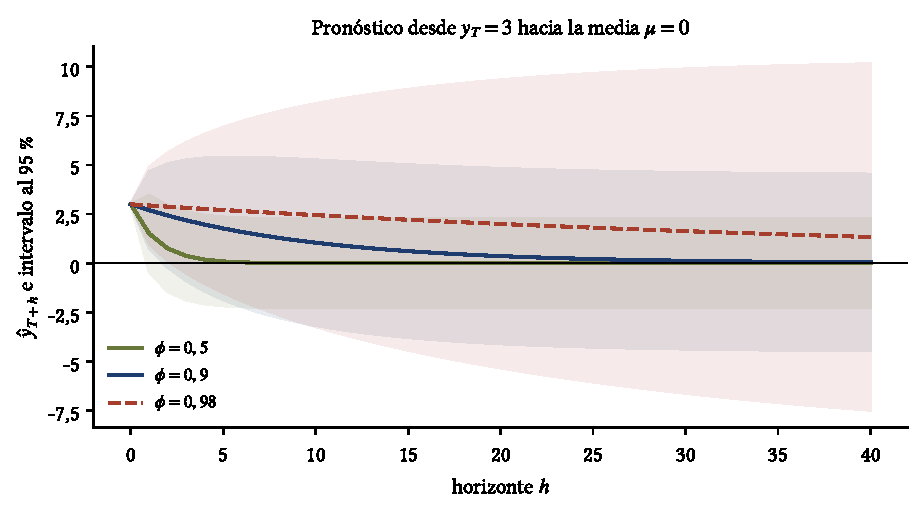
\includegraphics[width=0.78\linewidth]{graficos/cap06_fig_pronostico_ar1.pdf}
\caption{Pronóstico de un AR(1) desde $y_T=3$ con su intervalo al 95\,\% (bandas). Con $\phi=0{,}5$ el
pronóstico vuelve a la media en pocos períodos; con $\phi=0{,}98$ tarda mucho, y el intervalo se ensancha
hasta su límite $\pm1{,}96\,\sigma/\sqrt{1-\phi^2}$.}
\label{fig:pronar1}
\end{figure}

Para un ARMA(1,1), el pronóstico a un paso incorpora el último choque y los siguientes decaen como en el AR(1):
\begin{align*}
  \hat y_{T+1} &= \mu+\phi\,(y_T-\mu)+\theta\,\hat\varepsilon_T,\\
  \hat y_{T+h} &= \mu+\phi^{h-1}\,(\hat y_{T+1}-\mu),\\
  \E\bigl[(y_{T+h}-\hat y_{T+h})^2\bigr] &= \sigma^2\sum_{j=0}^{h-1}\psi_j^2,\qquad \psi_0=1,\quad \psi_j=\phi^{j-1}(\phi+\theta),
\end{align*}
donde los $\psi_j$ son los coeficientes de la representación $y_t=\mu+\sum_{j\ge0}\psi_j\varepsilon_{t-j}$.

\begin{definicion}[Prueba de Diebold-Mariano]
Para comparar dos pronósticos con errores $e_{1t}$ y $e_{2t}$, se define la diferencia de pérdidas
$d_t=e_{1t}^2-e_{2t}^2$ y el estadístico
\[
  DM=\frac{\bar d}{\sqrt{\hat S_d/n}},
\]
donde $\hat S_d$ es la varianza de largo plazo de $d_t$, estimada con Newey-West y $L=h-1$ rezagos (los errores
de pronóstico a $h$ pasos están autocorrelacionados hasta el rezago $h-1$). Bajo la hipótesis de igual
precisión, $DM\to N(0,1)$ (Diebold y Mariano, 1995).
\end{definicion}

% ---------------------------------------------------------------------
\section{Ejercicios resueltos}
% ---------------------------------------------------------------------

\begin{ejresuelto}{Identificación: los cambios de la tasa de interés a 10 años}\label{ej:tasaarma}
\enunciado Con los cambios mensuales del rendimiento del bono a 10 años (1953--2023): (a) calcule la ACF y la
PACF y proponga modelos candidatos; (b) estime AR(1), AR(2), MA(1), MA(2) y ARMA(1,1) por máxima verosimilitud
y compárelos con AIC y BIC; (c) relacione el resultado con el efecto de Working.

\solucion
\paso{Paso 1. ACF y PACF.} Con $T=845$, la banda al 95\,\% es $\pm0{,}067$. La ACF tiene un valor grande en el
primer rezago ($0{,}310$) y valores pequeños después; la PACF alterna de signo ($0{,}310$; $-0{,}212$;
$0{,}081$\ldots). El patrón ``ACF que se corta, PACF que decae alternando'' apunta a un MA(1)
(Figura~\ref{fig:identificacion}).

\paso{Paso 2. Comparación.} Los criterios de información, de menor a mayor (mejor primero):
\begin{center}\small
\begin{tabular}{@{}lrr@{}}
\toprule
Modelo & AIC & BIC \\
\midrule
MA(2)      & 17,45 & 36,41 \\
ARMA(1,1)  & 18,13 & 37,09 \\
MA(1)      & 23,27 & 37,49 \\
AR(2)      & 27,41 & 46,37 \\
AR(1)      & 64,33 & 78,55 \\
\bottomrule
\end{tabular}
\end{center}
Los dos criterios eligen el MA(2), pero las diferencias con el ARMA(1,1) y, para el BIC, con el MA(1) son
pequeñas. Los modelos autorregresivos puros quedan claramente atrás.

\paso{Paso 3. Working.} El MA(1) estimado tiene $\hat\theta=0{,}4454$, que implica
\begin{align*}
  \rho_1 &= \frac{\hat\theta}{1+\hat\theta^2}\\
         &= \frac{0{,}4454}{1+0{,}1984}\\
         &= \frac{0{,}4454}{1{,}1984}\\
         &= 0{,}372 .
\end{align*}
Si la tasa fuera un paseo aleatorio y solo se observara su promedio mensual, la Proposición~\ref{prop:workingma}
predice $\theta=0{,}268$ y $\rho_1=0{,}25$. La autocorrelación de los cambios mensuales se explica en buena
parte, aunque no del todo, porque la serie es un promedio de datos diarios.

\codigoweb{cap06_ej01}
\salidaR{cap06_ej01_R.txt}
\lectura{cap06_ej01}

\RvsPy \texttt{arima()} de R y \texttt{ARIMA} de \texttt{statsmodels} maximizan la misma verosimilitud exacta y
aquí coinciden en todas las cifras. Cambian los nombres: \texttt{ar1}, \texttt{ma1} e \texttt{intercept} en R;
\texttt{ar.L1}, \texttt{ma.L1} y \texttt{const} en Python. En los dos, la ``constante'' reportada es la
\emph{media} del proceso, no el término $c$ de la ecuación.

\begin{figure}[ht]
\centering
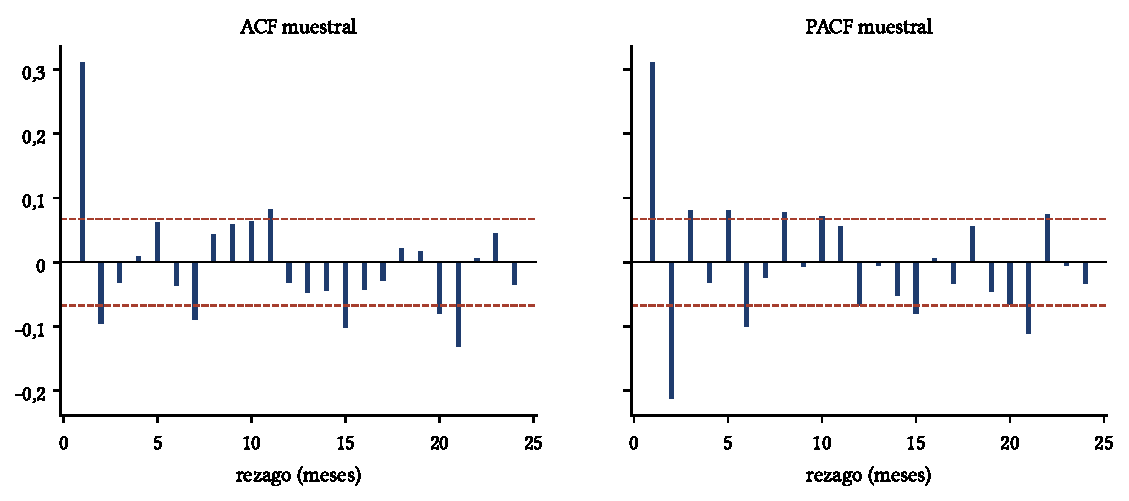
\includegraphics[width=0.92\linewidth]{graficos/cap06_fig_tasa_acf.pdf}
\caption{ACF y PACF muestrales de los cambios mensuales de la tasa a 10 años, con la banda al 95\,\%.}
\label{fig:tasaacf}
\end{figure}

\begin{conclusion}
Los cambios mensuales de la tasa a 10 años siguen aproximadamente un proceso de medias móviles de orden bajo.
Buena parte de esa dependencia es un artefacto de promediar: no es una oportunidad para predecir la dirección
de las tasas.
\end{conclusion}
\end{ejresuelto}

\begin{ejresuelto}{Estimación y diagnóstico: el logaritmo del VIX}\label{ej:vixarma}
\enunciado Estime AR(1), AR(2) y ARMA(1,1) para el logaritmo del VIX (1990--2026). Compare los criterios de
información, aplique la prueba de Ljung-Box a los residuos y calcule la vida media del modelo elegido.

\solucion
\paso{Paso 1. Selección.} AIC y BIC eligen el ARMA(1,1) ($-23\,678{,}75$ y $-23\,650{,}20$), con
$\hat\phi=0{,}9832$ y $\hat\theta=-0{,}0844$; ambos coeficientes son muy significativos
($\operatorname{ee}=0{,}0019$ y $0{,}0112$).

\paso{Paso 2. Diagnóstico.} Incluso en el mejor modelo, los residuos siguen autocorrelacionados:
$Q(10)=73{,}2$ con 8 grados de libertad, $p\approx10^{-12}$. Los demás modelos están peor. La
Figura~\ref{fig:vixresid} muestra que el AR(1) deja una autocorrelación negativa en los primeros rezagos, que
el ARMA(1,1) corrige en parte, pero quedan autocorrelaciones pequeñas y persistentes.

\paso{Paso 3. Vida media.}
\begin{align*}
  h^* &= \frac{\ln0{,}5}{\ln\hat\phi}\\
      &= \frac{-0{,}69315}{\ln0{,}9832}\\
      &= \frac{-0{,}69315}{-0{,}016943}\\
      &= 40{,}9 \text{ días}.
\end{align*}

\codigoweb{cap06_ej02}
\salidaR{cap06_ej02_R.txt}
\lectura{cap06_ej02}

\RvsPy Tres detalles hacen que las dos salidas sean comparables. Primero, \texttt{statsmodels} calcula por
defecto los errores estándar con el producto externo del gradiente; con \texttt{cov\_type="approx"} usa el
hessiano numérico, como R. Segundo, el primer residuo depende de cómo cada programa inicializa el filtro de
Kalman, así que lo excluimos en ambos. Tercero, los optimizadores difieren: $\hat\phi$ es $0{,}9832$ en R y
$0{,}9831$ en Python, lo que mueve la vida media entre $40{,}9$ y $40{,}6$ días. Diferencias de este tamaño son
normales en estimaciones no lineales y no cambian ninguna conclusión.

\begin{figure}[ht]
\centering
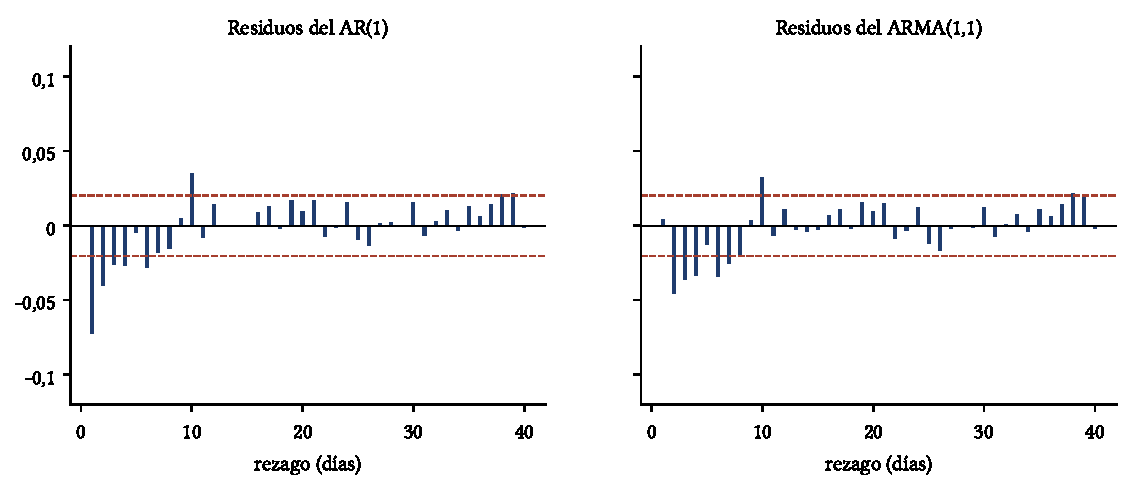
\includegraphics[width=0.92\linewidth]{graficos/cap06_fig_vix_resid.pdf}
\caption{ACF de los residuos del AR(1) y del ARMA(1,1) para el logaritmo del VIX, con la banda al 95\,\%.}
\label{fig:vixresid}
\end{figure}

\begin{conclusion}
El ARMA(1,1) es el mejor de los modelos ARMA de orden bajo para el VIX, pero no captura toda su dependencia,
en línea con la memoria larga detectada en el Ejercicio~\ref{ej:vixur}. Un modelo puede ser el mejor de los
candidatos y aun así ser inadecuado; el diagnóstico de residuos es lo que lo revela.
\end{conclusion}
\end{ejresuelto}

\begin{ejresuelto}{¿Supera el ARMA a un paseo aleatorio? Evaluación fuera de muestra}\label{ej:vixfuera}
\enunciado Estime el ARMA(1,1) del logaritmo del VIX con datos de 1990 a 2015. Con esos parámetros fijos,
pronostique a 1, 5 y 22 días desde cada día de 2016 a 2026, y compare con el paseo aleatorio (pronóstico igual
al último valor) y con la media de la muestra de estimación. Use la prueba de Diebold-Mariano.

\solucion
\paso{Paso 1. Parámetros.} Con datos hasta el 31 de diciembre de 2015: $\hat\mu=2{,}9228$, $\hat\phi=0{,}9861$ y
$\hat\theta=-0{,}0902$. Hay 2\,728 orígenes de pronóstico.

\paso{Paso 2. Precisión.} La raíz del error cuadrático medio (RECM), en puntos logarítmicos:
\begin{center}\small
\begin{tabular}{@{}rrrrrr@{}}
\toprule
$h$ & ARMA(1,1) & Paseo aleatorio & Media & ARMA/paseo & $DM$ \\
\midrule
1  & 0,0785 & 0,0792 & 0,3301 & 0,991 & 2,62 \\
5  & 0,1537 & 0,1579 & 0,3302 & 0,974 & 5,02 \\
22 & 0,2415 & 0,2630 & 0,3306 & 0,918 & 3,80 \\
\bottomrule
\end{tabular}
\end{center}
A 22 días, la mejora sobre el paseo aleatorio es de
\begin{align*}
  1-\frac{0{,}2415}{0{,}2630} &= 1-0{,}918\\
                              &= 0{,}082,
\end{align*}
es decir, un 8,2\,\% menos de error. A un día la mejora es menor del 1\,\%.

\paso{Paso 3. Significancia.} Los tres estadísticos $DM$ superan 1,96: el ARMA es significativamente más
preciso que el paseo aleatorio en los tres horizontes. Usar la media histórica es mucho peor que ambos.

\codigoweb{cap06_ej03}
\salidaR{cap06_ej03_R.txt}
\lectura{cap06_ej03}

\RvsPy Programamos la recursión de los residuos y los pronósticos a mano para que sean visibles las ecuaciones
de la sección de pronóstico. Las pequeñas diferencias en los parámetros (cuarta cifra decimal) se trasladan a
la tercera cifra del cociente a 5 días ($0{,}974$ frente a $0{,}973$) y a la segunda del estadístico $DM$.

\begin{figure}[ht]
\centering
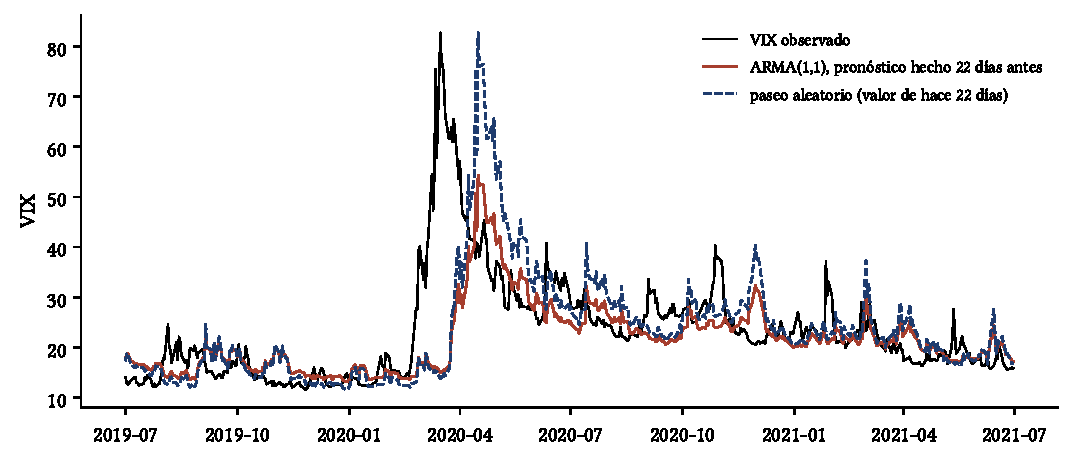
\includegraphics[width=0.92\linewidth]{graficos/cap06_fig_vix_pronostico.pdf}
\caption{Pronósticos a 22 días del VIX entre julio de 2019 y junio de 2021. Ningún modelo anticipa el salto de
marzo de 2020; después del salto, el ARMA(1,1) prevé la caída del VIX hacia su media, mientras que el paseo
aleatorio repite el nivel de crisis de 22 días antes.}
\label{fig:vixfuera}
\end{figure}

\begin{conclusion}
La reversión a la media del VIX es explotable para pronosticar: el ARMA(1,1) mejora al paseo aleatorio, sobre
todo a horizontes de un mes. Pero ningún modelo lineal anticipa los saltos; lo que hace mejor es prever su
disipación.
\end{conclusion}
\end{ejresuelto}

\begin{ejresuelto}{Pronóstico del VIX con intervalos de confianza}\label{ej:vixabanico}
\enunciado Con el ARMA(1,1) estimado con toda la muestra, pronostique el VIX desde el 22 de septiembre de 2026
hasta 60 días hábiles adelante, con intervalos al 95\,\%, y calcule el nivel de largo plazo.

\solucion
\paso{Paso 1. Pronóstico puntual.} El pronóstico del logaritmo es $\hat y_{T+h}=\hat\mu+\hat\phi^{h-1}(\hat y_{T+1}-\hat\mu)$,
y $e^{\hat y_{T+h}}$ es la mediana del pronóstico del VIX. Desde un nivel de 14,21, la mediana sube a 14,33
(1 día), 15,41 (22 días) y 16,70 (60 días), hacia el nivel de largo plazo
\begin{align*}
  e^{\hat\mu} &= e^{2{,}9042}\\
              &= 18{,}25 .
\end{align*}

\paso{Paso 2. Intervalos.} Con $\hat\sigma^2=0{,}004556$ y los pesos $\psi_j$, el intervalo al 95\,\% a 22 días es
$[9{,}50;\ 24{,}98]$ y a 60 días, $[8{,}98;\ 31{,}04]$. En el límite, el intervalo tiende a
$[9{,}39;\ 35{,}48]$.

\paso{Paso 3. Asimetría.} Los intervalos no son simétricos alrededor de la mediana: son simétricos en
logaritmos y, al exponenciar, la cola superior se alarga. Es coherente con la naturaleza del VIX, que puede
triplicarse en pocos días pero rara vez cae a la mitad.

\codigoweb{cap06_ej04}
\salidaR{cap06_ej04_R.txt}
\lectura{cap06_ej04}

\RvsPy Al final, la salida de Python compara nuestro cálculo con la función \texttt{get\_forecast} de
\texttt{statsmodels}, que reproduce la mediana a 22 días. En R se obtiene lo mismo con la función
\texttt{predict(m, n.ahead = 22)}.

\begin{figure}[ht]
\centering
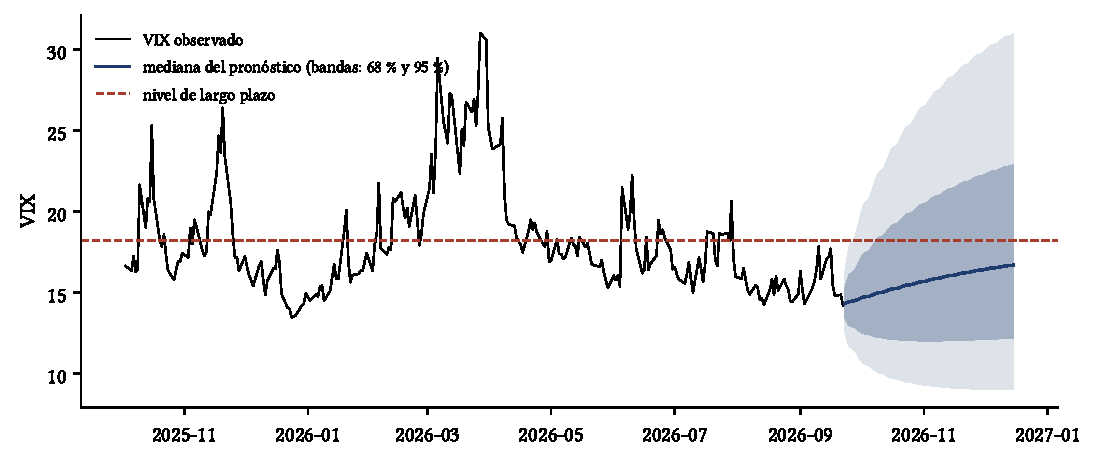
\includegraphics[width=0.92\linewidth]{graficos/cap06_fig_vix_abanico.pdf}
\caption{Último año del VIX y abanico de pronóstico a 60 días hábiles, con bandas al 68\,\% y al 95\,\%. La
mediana sube gradualmente hacia el nivel de largo plazo (línea discontinua), y la incertidumbre crece con el
horizonte, más hacia arriba que hacia abajo.}
\label{fig:vixabanico}
\end{figure}

\begin{conclusion}
Con un VIX por debajo de su media histórica, el modelo prevé un aumento gradual de la volatilidad implícita.
La amplitud del intervalo es la lección principal: a dos meses, valores entre 9 y 31 son compatibles con el
modelo.
\end{conclusion}
\end{ejresuelto}

\begin{ejresuelto}{El sesgo de Stambaugh en la predictibilidad de las acciones}\label{ej:stambaugh}
\enunciado Con datos mensuales de 1946 a 2023, estime la regresión del rendimiento total del S\&P 500 del mes
siguiente sobre $\ln(D_t/P_t)$ y el AR(1) del predictor. Calcule el sesgo de Kendall, el sesgo de Stambaugh y el
coeficiente corregido.

\solucion
\paso{Paso 1. Estimaciones.} Con $T=929$ meses: $\hat b=0{,}00611$ ($t=2{,}35$), aparentemente significativo
al 5\,\%; $\hat\phi=0{,}99759$; y la correlación entre las innovaciones es $-0{,}983$, con
$\hat k=\hat\sigma_{uv}/\hat\sigma_v^2=-0{,}9541$.

\paso{Paso 2. Sesgos.} Por la fórmula de Kendall y la Proposición~\ref{prop:stambaugh}:
\begin{align*}
  \text{sesgo de }\hat\phi &= -\frac{1+3\hat\phi}{T}\\
                           &= -\frac{1+3\times0{,}99759}{929}\\
                           &= -\frac{3{,}99277}{929}\\
                           &= -0{,}00430,\\
  \text{sesgo de }\hat b   &= \hat k\times(-0{,}00430)\\
                           &= -0{,}9541\times(-0{,}00430)\\
                           &= 0{,}00410 .
\end{align*}

\paso{Paso 3. Corrección.}
\begin{align*}
  \hat b_{\text{corregido}} &= \hat b-\text{sesgo de }\hat b\\
                            &= 0{,}00611-0{,}00410\\
                            &= 0{,}00201 .
\end{align*}
Dos tercios (67,1\,\%) del coeficiente estimado son sesgo. Además, como la fórmula de Kendall subestima el sesgo
cerca de la raíz unitaria (Figura~\ref{fig:kendall}), la corrección es conservadora: el coeficiente verdadero
probablemente es todavía menor.

\codigoweb{cap06_ej05}
\salidaR{cap06_ej05_R.txt}
\lectura{cap06_ej05}

\RvsPy El único cuidado es alinear las fechas: el rendimiento de $t$ a $t+1$ se regresa sobre la razón de $t$.
En R, \texttt{dp[-n]} quita el último valor y \texttt{dp[-1]} el primero; en Python, \texttt{dp[:-1]} y
\texttt{dp[1:]}.

\begin{figure}[ht]
\centering
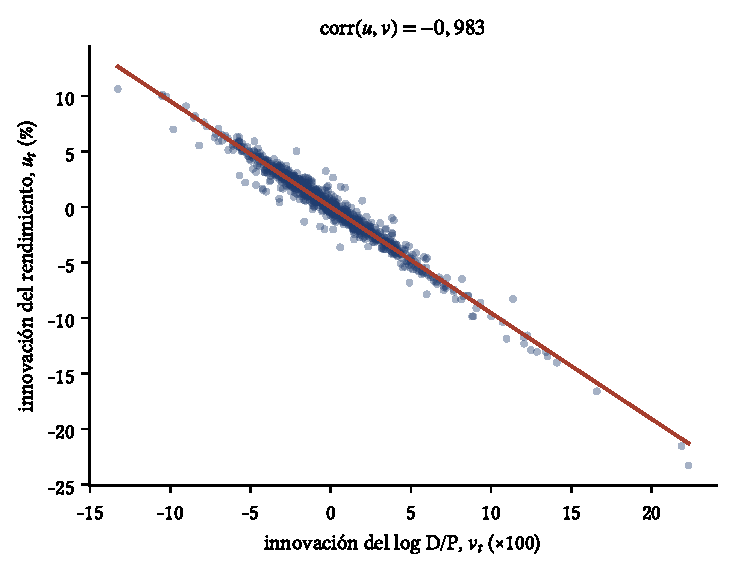
\includegraphics[width=0.62\linewidth]{graficos/cap06_fig_stambaugh.pdf}
\caption{Innovaciones del rendimiento frente a las del logaritmo de la razón dividendo/precio, 1946--2023. La
correlación es casi perfectamente negativa: cuando el mercado sube, la razón cae. Es esta relación, combinada con
la alta persistencia del predictor, la que produce el sesgo.}
\label{fig:stambaugh}
\end{figure}

\begin{conclusion}
La evidencia de predictibilidad con la razón dividendo/precio después de 1946 ($t=2{,}35$) es en buena parte un
sesgo de muestras finitas. Esta es la respuesta al Ejercicio propuesto~4.7: un estadístico $t$ alto no basta
cuando el predictor es muy persistente y sus innovaciones están correlacionadas con las del rendimiento.
\end{conclusion}
\end{ejresuelto}

% ---------------------------------------------------------------------
\section{Ejercicios propuestos}
% ---------------------------------------------------------------------

\begin{enumerate}[label=\textbf{\thechapter.\arabic*},leftmargin=*,itemsep=6pt]
  \item Derive la ACF de un MA(2) y demuestre que $\rho_j=0$ para $j\ge3$.
  \textit{Respuesta: $\rho_1=\theta_1(1+\theta_2)/(1+\theta_1^2+\theta_2^2)$, $\rho_2=\theta_2/(1+\theta_1^2+\theta_2^2)$.}

  \item Para el AR(2) con $\phi_1=1{,}2$ y $\phi_2=-0{,}5$, calcule $\rho_1$, $\rho_2$ y $\rho_3$, y las raíces de
  $1-1{,}2z+0{,}5z^2=0$. ¿Es estacionario? \textit{Respuesta: $\rho_1=0{,}8$, $\rho_2=0{,}46$, $\rho_3=0{,}152$;
  raíces $1{,}2\pm0{,}748i$, de módulo $1{,}414>1$.}

  \item Demuestre que el pronóstico de un paseo aleatorio a cualquier horizonte es el último valor observado y
  que su error cuadrático medio es $h\sigma^2$, que crece sin límite.

  \item Demuestre la fórmula de los pesos $\psi_j$ del ARMA(1,1) igualando coeficientes en
  $(1-\phi L)\sum_j\psi_jL^j=1+\theta L$.

  \item \emph{(Con datos.)} Repita el Ejercicio~\ref{ej:vixfuera} reestimando el ARMA(1,1) cada año (ventana
  creciente). ¿Mejora el pronóstico?

  \item \emph{(Con datos.)} Calcule la inflación mensual de EE.\,UU. desde 1953 con el IPC de la base de Shiller.
  Identifique un modelo ARMA. ¿Qué patrón aparece en el rezago 12 de la ACF y por qué?

  \item \emph{(Con datos del BCRP.)} Identifique y estime un modelo ARMA para la inflación mensual de Lima
  Metropolitana. Pronostique la inflación de los próximos 12 meses con intervalos y compárela con la meta de
  inflación del BCRP.

  \item \emph{(Simulación.)} Simule 2\,000 muestras con el modelo de la Proposición~\ref{prop:stambaugh},
  $b=0$, $\phi=0{,}99$, $T=300$ y $\operatorname{corr}(u,v)=-0{,}9$. ¿Con qué frecuencia rechaza la prueba $t$
  de $b=0$ al 5\,\% (a una cola)?
\end{enumerate}

% ---------------------------------------------------------------------
\section{Resumen de fórmulas}
% ---------------------------------------------------------------------

\begin{table}[H]
\centering\small
\begin{tabular}{@{}ll@{}}
\toprule
Concepto & Fórmula \\
\midrule
MA(1) & $\gamma_0=\sigma^2(1+\theta^2)$;\quad $\rho_1=\theta/(1+\theta^2)$;\quad $|\rho_1|\le1/2$ \\
Efecto de Working & $\theta=2-\sqrt3$ \\
AR(2) & $\rho_1=\phi_1/(1-\phi_2)$;\quad $\rho_j=\phi_1\rho_{j-1}+\phi_2\rho_{j-2}$ \\
ARMA(1,1) & $\rho_1=\frac{(1+\phi\theta)(\phi+\theta)}{1+2\phi\theta+\theta^2}$;\quad $\rho_j=\phi\rho_{j-1}$ \\
Sesgo de Kendall & $\E[\hat\phi]-\phi\approx-(1+3\phi)/T$ \\
Sesgo de Stambaugh & $\E[\hat b-b]=(\sigma_{uv}/\sigma_v^2)\,\E[\hat\phi-\phi]$ \\
Criterios de información & $\mathrm{AIC}=-2\hat\ell+2k$;\quad $\mathrm{BIC}=-2\hat\ell+k\ln T$ \\
Pronóstico AR(1) & $\hat y_{T+h}=\mu+\phi^h(y_T-\mu)$;\quad ECM $=\sigma^2(1-\phi^{2h})/(1-\phi^2)$ \\
Diebold-Mariano & $DM=\bar d/\sqrt{\hat S_d/n}\to N(0,1)$ \\
\bottomrule
\end{tabular}
\caption{Fórmulas principales del Capítulo 6.}
\end{table}

\section*{Referencias}
\begin{itemize}[leftmargin=*]
  \item Box, G. E. P. y Jenkins, G. M. (1970). \emph{Time Series Analysis: Forecasting and Control}.
        Holden-Day.
  \item Diebold, F. X. y Mariano, R. S. (1995). Comparing predictive accuracy. \emph{Journal of Business \&
        Economic Statistics}, 13(3), 253--263.
  \item Hamilton, J. D. (1994). \emph{Time Series Analysis}. Princeton University Press. Capítulos 3 a 5.
  \item Kendall, M. G. (1954). Note on bias in the estimation of autocorrelation. \emph{Biometrika},
        41(3--4), 403--404.
  \item Stambaugh, R. F. (1999). Predictive regressions. \emph{Journal of Financial Economics}, 54(3),
        375--421.
\end{itemize}
